This chapter contains the controller design for the refrigeration system model developed in \cref{sec:mod}. A simple pole-placement method controller will be made as an initial step to verify that the model is sufficient and to get a feel for the system before moving on to a more complex controller. An MPC controller is chosen due to its ability to handle constraints which is essential for handling the actuator limitations in a reefer system. Both the pole-placement and MPC controller will be benchmarked against the coupled PID controllers currently implemented at BITZER.


\subsection{State space controller - Pole placement}
The poles of a controllable state space system is the eigenvalues of the system matrix $(A)$. When the states of a state space system is fed back through a feedback gain $(K)$ the system matrix of the closed-loop system becomes:

\begin{equation} \label{eq:A_cl}
	A_{cl} = A-BK
\end{equation}

If \cref{fig:state_space_fb} is analyzed by looking at the how $\dot{x}$ is calculated from $x$ this becomes obvious. A controllable system has the appealing property of  pole placement. This means that in theory the poles of the system can be moved anywhere to achieve some specific behavior. Such a change could be to make the system faster by placing them further to the left in the complex plane.

\begin{figure}[h!]
	\centering
	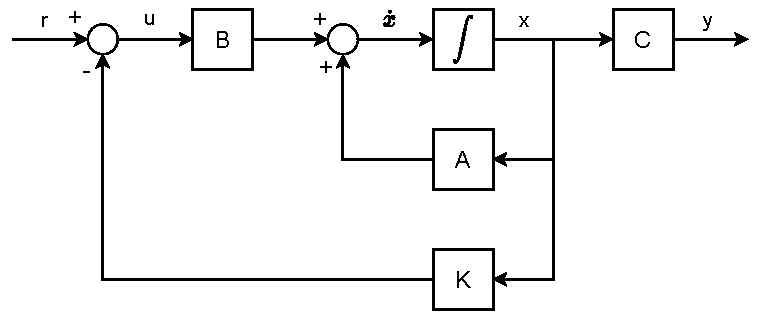
\includegraphics[width=0.60\textwidth]{Graphics/State_space_feedback.pdf}
	\caption{Generic state-space system with feedback}
	\label{fig:state_space_fb}
\end{figure}


% SIXO system pole placement algorithm
%For a \underline{SISO} system the poles can be placed by hand from the following algorithm:
%\begin{enumerate}
%	\item defining desired pole placements for all system poles and writing out the characteristic polynomial for these wanted system poles e.g.
%	$(s-p_1)(s-p_2) \cdots (s-p_n) = s^n + a_{cl_1} \cdot s^{n-1} + a_{cl_2} \cdot s^{n-2} \cdots a_{cl_n}$
%	\item calculating the eigenvalues of \cref{eq:A_cl} which yields the characteristic polynomial of the feedback system e.g.
%	$det(A_{sys}) = s^n + (a_{sys_1}-k_1) \cdot s^{n-1} + (a_{sys_2}-k_2) \cdot s^{n-2} \cdots (a_{sys_n}-k_n)$
%	\item setting the coefficients of the characteristic polynomial of the native system equal to the coefficients of the desired pole placement and solving for the entries in K e.g.
%	$ k_1 = a_{sys_1}-a_{cl_1}, k_2 = a_{sys_2}-a_{cl_2} \cdots k_n = a_{sys_n}-a_{cl_n} $
%	 This yields the $ K = [k_1, k_2 \cdots k_n]^T $ which places the poles at the desired location.
%	\item x is fed back through K to the input yielding \cref{eq:A_cl}.
%\end{enumerate}
%
%In Matlab the above algorithm can be performed by the simple function \textit{Place(A, B, poles)} where "A" is the system matrix, "B" the input matrix and "poles" an array of the desired poles. The \textit{place()} works for both SISO and MIMO systems.

In Matlab pole placement can be performed by the \textit{Place(A, B, poles)} function where "A" is the system matrix, "B" the input matrix and "poles" an array of the desired poles. The \textit{place()} function works for both SISO and MIMO systems.


\subsection{Linear Quadratic Regulator}
The first control strategy to be implemented is the infinite-horizon Linear Quadratic Regulator, referered to as the LQR controller. The LQR problem is an optimal control problem, that finds the optimal feedback gain, that will drive the states of a dynamical system to 0. This is done by selecting a control input u, that minimizes a relevant cost function. As an example consider the discrete-time system in \cref{eq:lqr_discrete_sys} with $x(k)$ representing the system states, $u(k)$ the control inputs and $y(k)$ the measured outputs.\\

\begin{equation} \label{eq:lqr_discrete_sys}
	\begin{split}
		\dot{x} 	& = Ax + Bu \\
		y 	& = Cx
	\end{split}
\end{equation}

A relevant cost function for this LQR problem would be on this form:

\begin{equation} \label{eq:lqr_cost_fcn}
	J = \int_0^{\infty} \left(x^TQx + u^TRu + 2x^TNu\right)dt
\end{equation}

where

\begin{center}
	\begin{tabular}{l r l }
		weight & $R$         & $ > 0$ (positive definite) and symmetric       \\
		weight & $Q$ and $N$ & $\ge 0$ (positive semi-definite) and symmetric
	\end{tabular}
\end{center}

The cross-term is typically ignored by defining $N=0$. The matrices Q and R are introduced to add weights to the various states and inputs. This allows the engineer to penalize critical states and inputs more than others. This is obviously generally useful, especially if deviations in certain states or inputs negatively impact the system energy consumption or could cause dangerous system behavior.\\
%The algorithm requires access to all system states, either through measurement or estimation. The latter is achieved by the linear model designed in \cref{sec:mod_lin}. \\

The value of Q and R is a choice the control engineer must make. While it in practicality requires some amount of trial-and-error iteration, there are methods for choosing a reasonable starting value. An often used tuning method to obtain initial Q and R matrices is following Bryson's rule. It states that the state x$_{\textit{i}}$ should be penalized by a factor $\dfrac{1}{\text{Max} \left(x_{\textit{i}}\right)^2}$. Similarly the control input u$_{\textit{i}}$ should be penalized by a factor $\dfrac{1}{\text{Max} \left(u_{\textit{i}}\right)^2}$. This effectively scales the maximum value of all entries in the cost function J to 1. This is particularly useful, when the states and inputs are have numerically large differences.\\


The fact that the LQR problem aims to set the states equal to zero, may sound like a undesirable goal. If a state is representative of a temperature measured in Kelvin, driving it to 0 is likely neither a realistic nor useful goal. However, lets recall the linearization of the system performed in \cref{sec:mod_lin}. The first order Taylor expansion did not only linearize the system, it also changed the psyical interpretation of the system states. Rather than being an absolute value, it is now the difference between the actual value and the equilibrium point used for linearization. This means that the LQR problem will seek to set this difference to 0, thus driving the system to the equilibrium point.\\

Thus the cost function with no cross-term cost becomes:

\begin{equation} \label{eq:lqr_cost_fcn}
	J = \int_0^{\infty} \left( \bar{x}^TQ\bar{x} + \bar{u}^TR\bar{u} \right)dt
\end{equation}

with $\bar{x} = x-x_o$ and $\bar{u} = u-u_o$ where $x_o$, $u_o$ are the linearisation equilibrium operating points of the states and inputs.

The optimal feedback gain K can be shown to be

\begin{equation} \label{eq:lqr_K}
	K = R^{-1}B^{T}P
\end{equation}

where P is the unique solution to the algebraic Ricatti equation 
\begin{equation} \label{eq:ricatti}
	A^TP + PA - PBR^{-1}B^TP+Q = 0
\end{equation}

While proving \cref{eq:lqr_K} explicitly is beyond the scope of this report, it is noted that it is found by following Pontryagin's minimum principle. Briefly described the process is to first define the Hamiltonian associated with the optimization problem. Differentiating the Hamiltonian with respect to the control signal u, yields the control gradient. By then setting the gradient equal to 0 and solving for u, the optimal control input is found.
\\


LQR is chosen as the initial control strategy due to its intuitive way of use, as well the many proven properties. These include a gueranteed 6dB gain- and $60^\circ$ phase margin.

\subsubsection{Integral action}
In most control problems it is often the goal to keep an output at a reference value. The methods of achiving this are many, but the most commonly used are reference scaling and integral action. Reference

LQR does not inherently have integral action, in the definition that it does not drive the output to a reference value. As stated previously, it attempts to set the states to zero. The common way to include integral action in state space controllers is to extend the state vector, with one or more artificial integral states.
 \begin{equation} \label{eq:ricatti}
 	\tilde{x} = \begin{bmatrix}
 		x \\ x_i
 	\end{bmatrix}
 \end{equation}

where $x_i = y-r$.\\

This approach allows the user to set a reference for this state, and design a controller that minimizes the difference between the two. If the reference for $x_i$ is 0, the controller will set $x_i = 0$, which satisfies $y = r$. This poses a conflicting objective for the LQR algorithm however, as it will attempt to set \textit{all} states equal to zero. Since y is a linear function of the state vector $y = Cx$, where x is already being driving to zero, requiring $y=r$ is only sensible if $r=0$.
Instead one must perform a state transformation to a coordinate system, where $x=0$ satisfies $y=r$. Here, we again reap the benefits of the linearisation performed when obtaining the system model. In this linearisation the origin of the state space was moved from 0 to an operating point. The result is that achieving $$

\subsection{LMI / MPC controller}
Model Predictive Control (MPC) is, like the Linear Quadratic Regulator, an optimal control algorithm with respect to some cost function. It is optimal with regards to the current sample but in contrast to LQR it also takes future samples into account. It relies on a dynamic model of the controlled process and is able to consider various types of constraints.\\

At every time sample the MPC controller
\begin{enumerate}
	\item optimizes over \textit{prediction horizon} $(H_p)$
	\item calculates a predictive optimal control trajectory
	\item applies the first sample in the predicted control trajectory to the process
\end{enumerate}

\medskip

Consider the discrete-time system in \cref{eq:mpc_discrete_sys}. While $y(k)$ represents the measured outputs, $z(k)$ represents the controlled non-measured outputs. It is possible that $y(k) = z(k)$ in this case all controlled outputs are measured.

\begin{equation} \label{eq:mpc_discrete_sys}
	\begin{split}
		x(k+1) 	& = Ax(k) + Bu(k) \\
		y(k) 	& = C_yx(k) \\
		z(k) 	& = C_zx(k)
	\end{split}
\end{equation}

For such a system the MPC controller optimizes with respect to the quadratic cost function in \cref{eq:mpc_cost_fcn}. The first part of the cost function seeks to minimize the deviation of the controlled states $(\hat{z})$ from the reference trajectory $(r)$ over the prediction horizon where $Q(i)$ are the weights applied at each predicted sample. The second part insures integral action by minimizing change in control input $(\Delta \hat{u})$ (control moves) over the \textit{control horizon} $(H_u)$ where $R(i)$ are the weights applied to each control move into the future.

\begin{equation} \label{eq:mpc_cost_fcn}
	V(k) = \sum_{i=H_w}^{H_p}||\hat{z}(k+i|k) - r(k+i|k)||^2_{Q(i)} + \sum_{i=0}^{H_u-1}||\Delta \hat{u}(k+i|k)||^2_{R(i)}
\end{equation}

where

\begin{center}
	\begin{tabular}{l r l }
		                   & $||x||_M$               & $= \sqrt{\left(w^TMw\right)}$         \\
		prediction horizon & $H_p$                   & $\ge$ $H_u$ control horizon           \\
		window horizon     & $H_p$                   & $\ge 1$                               \\
		weights            & $Q(i), R(i)$            & $\ge 0$ (positive semi-definite)      \\
		control move       & $\Delta \hat{u}(k+i|k)$ & $= \hat{u}(k+i|k) - \hat{u}(k+i-1|k)$
	\end{tabular}
\end{center}

$Q(i), Q(i), H_p, H_u, H_w$ are considered the MPC tuning parameters.\\

An important characteristic of MPC is the ability to include constraints. Constraints can be applied to \textit{actuator slew rate}, \textit{actuator range} and \textit{controlled variables}. These constraints need to be formulated in the correct manner as seen below:

\begin{itemize}
	\item Actuator slew rate:

	\begin{equation} \label{eq:mpc_const_sr}
		E \begin{bmatrix} \Delta U(k) \\ 1 \end{bmatrix} \le 0
	\end{equation}
	\begin{center} where \end{center}
	\begin{equation*}
		\Delta U(k) = [\Delta \hat{u}(k|k)^T \cdots \Delta \hat{u}(k+H_u-1|k)^T]^T
	\end{equation*}


	\item Actuator range:

	\begin{equation} \label{eq:mpc_const_ar}
		F \begin{bmatrix} U(k) \\ 1 \end{bmatrix} \le 0
	\end{equation}
	\begin{center} where \end{center}
	\begin{equation*}
		U(k) = [\hat{u}(k|k)^T \cdots \hat{u}(k+H_u-1|k)^T]^T
	\end{equation*}

	\item Controlled variable

	\begin{equation} \label{eq:mpc_const_cv}
		G \begin{bmatrix} Z(k) \\ 1 \end{bmatrix} \le 0
	\end{equation}
	\begin{center} where \end{center}
	\begin{equation*}
		Z(k) = [\hat{z}(k+H_w|k)^T \cdots \hat{z}(k+H_p|k)^T]^T
	\end{equation*}
\end{itemize}

\noindent with E, F and G having appropriate dimensions.






